\problemname{Moving Boxes}

You have just helped a friend move, but unfortunately you got stuck at
the wrong end of a narrow corridor full of moving boxes. The corridor
consists of $N$ stacks of moving boxes, where stack number $i$
contains $a_i$ boxes. All boxes are the same size.

The only way to get out is to walk on top of the stacks from stack
$1$ to stack $N$. If you are on a stack, you can walk to an
adjacent stack, but only if it is not taller than the one you are standing on.
If the stack you are standing on is at least two boxes taller than an adjacent
stack, you can also push the top box off the stack you are standing on onto the adjacent stack. This can be repeated any number of times.

You are currently on stack $1$. Unfortunately, it might be impossible
for you to reach stack $N$. But luckily, you may add any number of
{\em extra} boxes to stack $1$ before you start walking. Write a program that
calculates how many extra boxes you need to add in order to reach stack $N$.

\begin{figure}[!h]
\begin{center}
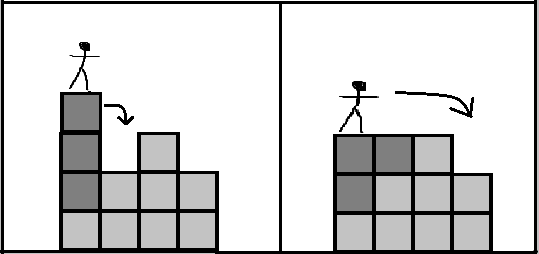
\includegraphics[width=8cm]{kartongbild2.png}
\end{center}
\caption{The figure shows sample 1. The dark gray boxes are extra boxes. The strategy is to push the top extra box onto stack 2. After that, you can walk straight to stack 4. It would not have worked with fewer than 3 extra boxes.}
\end{figure}

\section*{Input}
The first line contains an integer $N$, the number of stacks. The second line contains $N$ integers $a_i$, the number of boxes in each stack.

\section*{Output}
The program shall output one integer: the minimum number of extra moving boxes that need to be added.


\section*{Scoring}

For test cases worth
\begin{tabular}{llll}
$20$ points & it holds that &$N=3$ & , $1 \le a_i \le 20$. \\
$20$ points &  & $3\le N\le 5$ & , $1 \le a_i \le 100$.\\
$20$ points &  & $5\le N\le 10$ & , $1 \le a_i \le 1000$. \\
$40$ points &  & $10\le N\le 20$ &, $1 \le a_i \le 3000$. \\
\end{tabular}
